\title{LEZIONE 6 18/03/2020}\newline
\textbf{link} \href{https://web.microsoftstream.com/video/0c2093a0-44b9-4c83-a0b1-7e61fbd111b5?list=user&userId=faa91214-a6f5-40d7-8875-253fd49b8ce1}{clicca qui}
\subsection{Teorema del valore iniziale}
\[
    V(s) = \mathcal{L}[v(t)] \Longrightarrow v(0) = \lim_{s\rightarrow \infty}s V(s)
\] 
dove possiamo usare $v(0^+)$ se $v$ è discontinua in $0$.\newline
\newline
\textbf{es.} dato $v(t) = sca(t)$, la sua trsformata è $V(s) = \frac{1}{s}$ e $v(0^+) = 1$ perchè $\lim_{s\rightarrow \infty}s \cdot \frac{1}{s} = 1$.
\subsection{Teorema del valore finale}
\[
    V(s) = \mathcal{L}[v(t)] \Longrightarrow \text{se esiste}\; \lim_{t\rightarrow \infty} v(t) \text{, allora}\;\lim_{t\rightarrow \infty} v(t) = \lim_{s\rightarrow 0}sV(s)
\]
\subsection{Trasformate di Laplace notevoli}
\renewcommand{\arraystretch}{2}
\begin{center}
    \begin{tabular}{ |c|c| } 
     \hline
     \;\;\;\;\;\;\;\;\;\;\;\;\;\;\;$v(t)$ \;\;\;\;\;\;\;\;\;\;\;\;\;\;\;& \;\;\;\;\;\;\;\;\;\;\;\;\;\;\;$V(s)$ \;\;\;\;\;\;\;\;\;\;\;\;\;\;\;\\ 
     \hline
     $k \cdot imp(t)$ & $k \cdot 1$ \\ 
     $k \cdot sca(t)$ & $k \cdot \frac{1}{s}$  \\ 
     $k \cdot ram(t) =k \cdot t \cdot  sca(t)$ & $k \cdot \frac{1}{s^2}$ \\
     $k \cdot e^{at}sca(t)$ & $k \cdot \frac{1}{s-a}$ \\ 
     $t^{n}\cdot e^{at}sca(t)$ & $\frac{n!}{(s-a)^{n+1}}$\\ 
     \hline
    \end{tabular}
\end{center}
\renewcommand{\arraystretch}{1}
\textbf{oss.} Da notare è che la rampa è l'integrale dello scalino, che a sua volta è l'integrale dell'impulso (vedi trasformata di Laplace dell'integrale). Queste prime tre trasformate fanno parte di un gruppo di segnali che prendono il nome di \textbf{segnali canonici}, e sono tutte quelle trasformate di Laplace che valgono $\frac{1}{s^n}$.\newline
\newline
\textbf{oss.}  Notiamo che i segnali trigonometrici sono rappresentabili come esponenziali complessi, per esempio $sin(\omega t) = \frac{e^{j \omega t}- e^{-j \omega t}}{2j} \dots$ e così possiamo ricavare le trasformate di Laplace di tutte le funzioni trigonometriche.
\subsection{Antitrasformazione secondo Heaviside}
Questo metodo vale per trasformate di Laplace razionali fratte, cioè trasformate che possono essere scritte come
\[
    V(s) = \frac{N(s)}{D(s)}
\] dove $N, D$ sono polinomi in $s$; inoltre \textbf{il grado di $N$ è sempre minore o uguale al grado di $D$}.\newline
\newline
Il meccanismo di antitrasformazione di Heaviside consiste nella scomposizione di $V(s)$ in una somma di fratti semplici la cui $\mathcal{L}^{-1}$ è nota.\newline
\newline
Vediamo un esempio per capire il meccanismo dell'antitrasformata secondo Heaviside, successivamente esporremo il metodo generale.\newline
\newline
\textbf{es.} sia la trasfromata di Laplace $V(s) = \frac{s+2}{s(s+1)(s+3)}$, per antitrasformarla scrivo $V(s) = \frac{\alpha}{s} + \frac{\beta}{s+1} + \frac{\gamma}{s+3}$, a questo punto devo calcolare $\alpha, \beta$ e $\gamma$ facendo il denominatore comune ed eguagliando i numeratori:
\[
    \alpha(s+1)(s+3) + \beta s(s+3) + \gamma s (s+1) = s+2
\]
e ora mi basta eguagliare i coefficienti dei vari gradi di $s$ in modo da avere un sistema con cui trovare $\alpha, \beta$ e $\gamma$, oppure, più semplicemente, mi basta notare che imponento $s=0, s=-1$ e $s=-3$ deduco che:
\[
    \begin{cases}
        s=0 \Rightarrow 3 \alpha = 2 \Rightarrow  \alpha = \frac{2}{3}\\
        s = -1 \Rightarrow \beta = - \frac{1}{3}\\
        s = -3 \Rightarrow \gamma = - \frac{1}{6}
    \end{cases}
\]
Quindi $V(s) = \frac{2/3}{s} - \frac{1/2}{s+1} - \frac{1/6}{s+3}$ di cui so fare l'antitrasformata sfruttando le trasformate notevoli:
\[
    \mathcal{L}^{-1} = \frac{2}{3}sca(t) - \frac{1}{2}e^{-t}sca(t) - \frac{1}{6}e^{-3t}sca(t)
\]
\rule{\textwidth}{0,4pt}
\newline
\newline
Vediamo ora il \textbf{caso generale}:\newline
Sia
\[
    V(s) = \frac{N(s)}{D(s)}
\]
una trasformata di Laplace, con $N,D$ polinomi in $s$.\newline
\newline
Le radici di $N(s)$ prendono il nome di \textbf{zeri} della trasformata di Laplace, mentre le radici di $D(s)$ prendono il nome di \textbf{poli} della trasformata di Laplace.\newline
\newline
Il primo passaggio è quello di fattorizzare $D(s)$, che risulterà così espresso come prodotto di termini del tipo $s-p$ (dove quindi sarà presente un polo reale semplice) oppure $(s-p)^n$ (dove quindi sarà presente un polo reale multiplo) oppure altri casi complessi che però non tratteremo.
\begin{itemize}
    \item \textbf{Polo reale semplice}:\newline
    La trasformata è della forma 
    \[
        \frac{N(s)}{\dots(s-p)\dots} =
    \]
    (al denominatore ci possono essere vari fattori, l'importante è che ci sia il fattore $(s-p)$), la scomposizione è della forma
    \[
        = \dots + \frac{\alpha}{s-p} + \dots
    \]
    \item \textbf{Polo reale multiplo}:\newline
    La trasformata è della forma
    \[
        \frac{N(s)}{\dots (s-p)^n \dots} =
    \]
    la scomposizione è della forma
    \[
        = \dots + \frac{\alpha_1}{s-p} + \frac{\alpha_2}{(s-p)^2} + \dots + \frac{\alpha_n}{(s-p)^n} + \dots
    \]
    \item \textbf{Casi complessi}: [non li vediamo nel corso]
\end{itemize}
A seguito della scomposizione l'antitrasformata di Laplace è facilmente calcolabile usando le trasformate di Laplace notevoli.
\newline
\newline
\newline
\textbf{es.} dato $V(s) = \frac{2}{(s-1)^2(s+2)}$, trovare $v(t)$:\newline
Scompongo la trasformata:
\[
    V(s) = \frac{\alpha}{s-1} + \frac{\beta}{(s-1)^2} + \frac{\gamma}{s+2}
\]
Denominatore comune ed eguaglio i numeratori:
\[
    \alpha(s-1)(s+2) + \beta(s+2) + \gamma(s-1)^2 = 2
\]
Per trovare $\alpha, \beta$ e $\gamma$ ci sono due possibilità, o svolgo tutte le moltiplicazioni dell'equazione precedente e poi costruisco un sistema eguagliando i coefficienti dei vari $s^0, s^1, s^2, \dots$, oppure più semplicemente cerco i poli che sono $1$ e $-2$ e ricavo $\alpha, \beta$ e $\gamma$ sostituendoli in $s$:
\[
    \begin{cases}
        s=1 \Rightarrow 3 \beta = 2 \Rightarrow \beta = \frac{2}{3}\\
        s=-2 \Rightarrow 9 \gamma = 2 \Rightarrow \gamma = \frac{2}{9}\\
        s=[\text{qualunque numero a piacere, per esempio 0}] = 0 \Rightarrow \\
        \text{\;\;\;\;\;} \Rightarrow \text{usando i valori precedentemente trovati di $\beta$ e $\gamma$}\; \Rightarrow \alpha=-\frac{2}{9} 
    \end{cases}
\] 
Quindi
\[
    V(s) = \frac{-2/9}{s-1} + \frac{2/3}{(s-1)^2} + \frac{2/9}{s+3}
\]
\[
    \mathcal{L}^{-1}[V(s)] = v(t) = -\frac{2}{9} e^{t} sca(t) + \frac{2}{3} t e^{t} sca(t) + \frac{2}{9}e^{-2t} sca(t)
\]
\rule{\textwidth}{0,4pt}
\newline
\newline
\textbf{es.}\newline
[immagine dagli appunti del prof]
\begin{center}
    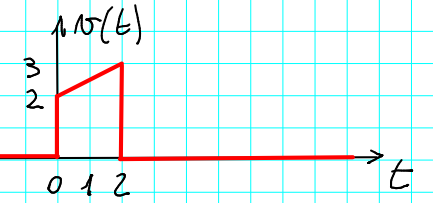
\includegraphics[height=3cm]{../lezione6/img1.PNG}
\end{center}
Cerchiamo di scrivere il segnale $v(t)$ a partire dal suo grafico in una somma di segnali canonici eventualmente ritardati.\newline
Ogni volta che c'è un cambio di pendenza interviene una rampa.\newline
\[
    v(t)= 2 sca(t) + 0,5 ram(t) - 3 sca(t-2) - 0,5 ram(t-2)
\] 
\[
    V(s) = \frac{2}{s} + \frac{0,5}{s^2} - \frac{3}{s}e^{-2s} - \frac{0,5}{s^2}e^{-2s} 
\]
\newpage
\section{Funzione di trasferimento}
Lavoriamo con SD LTI a TC SISO.
\subsection{Trasformata di Laplace delle equazioni di stato e d'uscita}
\subsubsection{Equazione di stato}
\[
    \begin{cases}
        \dot{x} = Ax + bu\\
        y = cx + du
    \end{cases} \;\;\;\; \text{rappresentamento di stato}\;
\]
\newline
Trasformiamo secondo Laplace l'\textbf{equazione di stato}:
\[
    \mathcal{L}[\dot{x}(t)] = \mathcal{L}[Ax(t) + bu(t)]
\]
Usiamo ora la proprietà della derivata e la proprietà di linearità della trasformata di laplace:
\[
    sX(s)-x(0) = AX(s) + bU(s)
\]
che posso riscrivere come
\[
    (sI-A)X(s) = x(0) + bU(s)
\]
Allora per qualunque $s$ che appartiene all'insieme degli autovalori di $A$ posso scrivere:
\[
    X(s) = (sI-A)^{-1} x(0) + (sI-A)^{-1} bU(s)
\]
La trasformata di Laplace dell'equazione di stato è quindi composta da due termini: il primo dipende linearmente solo dallo stato iniziale, il secondo dipende linearmente solo dall'ingresso.\newline
Quindi il primo termine $(sI-A)^{-1} x(0)$ è la trasformata di Laplace del \textbf{movimento libero (ML)} di $x$, e il secondo termine $(sI-A)^{-1} bU(s)$ è la trasformata di Laplace del \textbf{movimento forzato (MF)} di $x$.\newline
\newline
\textbf{oss.} Questa formula che abbiamo scritto è la corrispondente nel dominio delle trasformate di ciò che nel dominio del tempo è la \textbf{formula di Lagrange} dello stato.
\subsubsection{Equazione d'uscita}
Ora trasformiamo l'\textbf{equazione d'uscita} e vi sostituiamo $X(s)$ che calcolato precedentemente:
\[
    Y(s) = cX(s) + dU(s) = c(sI-A)^{-1} x(0) + [c(sI-A)^{-1} b + d]U(s)
\]
Anche qui il primo termine $c(sI-A)^{-1} x(0)$ è la trasformata di Laplace del \textbf{movimento libero (ML)} di $y$, e il secondo termine $[c(sI-A)^{-1} b + d]U(s)$ è la trasformata di Laplace del \textbf{movimento forzato (MF)} di $y$.\newline
\newline
Il movimento forzato contiene al suo interno il fattore $c(sI-A)^{-1} b$, che prende il nome di \textbf{funzione di trasferimento} $G(s)$. La funzione di trasferimento è il termine che moltiplicato per la trasformata dell'ingresso ti restituisce il movimento forzato.\newline
\newline
\newline
Riassunto per SD LTI a TC SISO:
\begin{itemize}
    \item Descrizione nello spazio di stato: quaterna $A, b, c, d$.
    \item Descrizione ingresso/uscita: funzione di trasferimento (FdT) $G(s) = c(sI-A)^{-1}b +d$.
    \item Interpretazione: $\mathcal{L}[\text{uscita forzata da u(t)}]= G(s) \mathcal{L}[u(t)]$ 
\end{itemize}
\subsection{Calcolo e aspetto di una funzione di trasferimento}
\[
    \text{Funzione di trasferimento:}\;\; G(s) = c(sI-A)^{-1} b +d
\]
Come è fatta? Analiziamone la struttura.\newline
\newline
Analiziamo prima il solo termine
\[
    (sI-A)^{-1} = \frac{1}{det(sI-A)} \left[\begin{matrix}
        \Delta_{11}(s) & \dots & \Delta_{1n}(s)\\
        \dots & \dots & \dots \\
        \Delta_{n1}(s) & \dots & \Delta_{nn}(s)
    \end{matrix}\right]
\] 
dove il denominatore $det(sI-A)$ è il polinomio caratteristico di $A$, che quindi ha grado $n$ (= ordine del sistema); e dove i termini $\Delta_{ik}(s)$ sono determinanti di matrici $(n-1)\text{x}(n-1)$ e quindi hanno grado al più $n-1$.\newline
\newline
Vediamo ora il termine
\[
    c(sI-A)^{-1} b = \frac{1}{det(sI-A)} \left[\begin{matrix}
        c_1 & \dots & c_n
        \end{matrix}\right] \{\Delta_{ij}(s)\}\left[\begin{matrix}
            b_1\\
            \dots\\
            b_n
    \end{matrix}\right]
\], dove $\{\Delta_{ij}(s)\} = \left[\begin{matrix}
    \Delta_{11}(s) & \dots & \Delta_{1n}(s)\\
    \dots & \dots & \dots \\
    \Delta_{n1}(s) & \dots & \Delta_{nn}(s)
\end{matrix}\right]$ come al punto precedente. Ancora una volta otteniamo un polinomio di al più grado $n-1$.\newline
\newline
Vediamo ora il termine finale $G(s)$
\[
    G(s) = c(sI-A)^{-1} b +d = \frac{\bar{N}(s)}{D(s)} +d
\]
dove il termine $c(sI-A)^{-1} b$ ci riconduce a un'espressione razionale fratta $\frac{\bar{N}(s)}{D(s)}$, con $D(s)$ polinomio caratteristico di $A$ e quindi grado $n$, e invece $\bar{N}(s)$ è un polinomio di grado al più $n-1$.\newline
\newline
Se e solo se $d=0$ (cioè se il sistema è strettamente proprio) abbiamo $G(s) = \frac{\bar{N}(s)}{D(s)}$ in cui il grado del numeatore è minore del grado del denominatore.\newline
Altrimenti (se e solo se $d\neq 0$) abbiamo $G(s) = \frac{\bar{N}(s) + dD(s)}{D(s)} = \frac{N(s)}{D(s)}$, con $N(s) = \bar{N}(s) +dD(s)$, in cui il grado del numeratore è uguale al grado del denominatore.\newline
\newline
Quindi, riassumendo,
\begin{itemize}
    \item $G(s)$ è razionale fratta.
    \item I suoi poli (radici del denominatore) sono autovalori di $A$.\newline
    \textbf{oss.} In alcuni casi può darsi che non tutti gli autovalori di $A$ compaiano come poli, perchè capita che alcuni termini del numeratore si semplifichino col alcuni termini del denominatore (ci torneremo più avanti).
    \item Il grado del numeratore è uguale al grado del denominatore se e solo se ($\Leftrightarrow$) $d\neq 0$, altrimento il grado del numeratore è minore ($<$) del grado del denominatore.
\end{itemize}
\subsection{Esempi}
\textbf{es.}  Dato il Sd LTI a TC SISO descritto nello spazio di stato da 
\[
    A=\left[\begin{matrix}
        1 & -1\\
        3 & 4
    \end{matrix}\right] \;\;\;\;\; b = \left[\begin{matrix}
        1\\0
    \end{matrix}\right] \;\;\;\;\; c= \left[\begin{matrix}
        2 &1
    \end{matrix}\right] \;\;\;\;\;d=0
\]
calcolare la funzione di trasferimento $G(s)$.
\[
    G(s) = c (sI-A)^{-1} b +d = \left[\begin{matrix}
        2 &1
    \end{matrix}\right]\left[\begin{matrix}
        s-1&1\\
        -3 & s-4
    \end{matrix}\right]^{-1} \left[\begin{matrix}
        1\\0
    \end{matrix}\right]+0 = 
\]
[esiste un trucchetto per calcolare la trasposta della generica matrice $M$ 2x2: si moltiplica $\frac{1}{det(M)}$ per la matrice ottenuta scambiando di posto i termini sulla diagonale principale e invertendo il segno dei termini sulla diagonale secondaria]
\[
    = \frac{1}{(s-1)(s-4) +3} \left[\begin{matrix}
        2&1
    \end{matrix}\right]\left[\begin{matrix}
        s-4 & -1\\
        3 & s-1
    \end{matrix}\right]\left[\begin{matrix}
        1\\0
    \end{matrix}\right]=
\]
\[
    \frac{1}{s^2 -5s +7} \left[\begin{matrix}
        2&1
    \end{matrix}\right]\left[\begin{matrix}
        s-4\\3
    \end{matrix}\right] = \frac{2s -5 }{s^2 -5s +7}
\]